\documentclass[10pt,twocolumn,letterpaper]{article}

% --- Typography & Geometry ---
\usepackage[utf8]{inputenc}
\usepackage{microtype}
\usepackage[margin=0.75in,top=0.85in,bottom=0.85in]{geometry}

% --- Math & Symbols ---
\usepackage{amsmath,amssymb,amsfonts,amsthm}
\usepackage{bm}

% --- Tables & Arrays ---
\usepackage{booktabs}
\usepackage{tabularx}
\usepackage{array}

% --- Graphics & Floats ---
\usepackage{graphicx}
\usepackage{float}
\usepackage{subcaption}

% --- Code Listings ---
\usepackage{xcolor}
\usepackage{listings}

\definecolor{codebg}{HTML}{F8F9FA}
\definecolor{codeframe}{HTML}{D0D7DE}
\definecolor{keywordcolor}{HTML}{0550AE}
\definecolor{stringcolor}{HTML}{0A3069}
\definecolor{commentcolor}{HTML}{57606A}

\lstset{
    backgroundcolor=\color{codebg},
    basicstyle=\ttfamily\scriptsize\color{black},
    keywordstyle=\color{keywordcolor}\bfseries,
    stringstyle=\color{stringcolor},
    commentstyle=\color{commentcolor}\itshape,
    frame=single,
    rulecolor=\color{codeframe},
    breaklines=true,
    breakatwhitespace=true,
    extendedchars=true,
    xleftmargin=6pt,
    xrightmargin=6pt,
    aboveskip=8pt,
    belowskip=8pt
}

% --- Hyperlinks ---
\usepackage{hyperref}
\hypersetup{
    colorlinks=true,
    linkcolor=blue!70!black,
    citecolor=blue!70!black,
    urlcolor=blue!70!black
}

% --- Input Title & Authors ---
% Metadata for leka_v2
\title{\textbf{LEKAv2: Linear-Time Efficient Kernel Attention with Landmark Distillation}}

\author{
  \textbf{Taha Majs}\thanks{Corresponding author: tahamajs@uni.edu} \quad \textbf{Research Team} \\
  Department of Computer Science \\
  Advanced Machine Learning \& Efficiency Laboratory
}

\date{\today}


\begin{document}

\maketitle

% --- Abstract & Keywords Block ---
\begin{abstract}
Linear attention scales as $\mathcal{O}(L)$ in sequence length by replacing 
softmax with a kernel feature map, but achieves this at the cost of 
\textbf{uniform aggregation}: every query attends to the full aggregated 
KV state, losing the ability to selectively focus on important 
positions. We introduce \textbf{LEKAv2}, which extends the linear-attention 
primitive with \textbf{landmark distillation} and **learned local-global 
fusion**:

\begin{enumerate}
\item \textbf{Dual-scale random features.} We map Q/K through two independent
  RFF projections ($F$ and $F/2$ dimensions) and concatenate the
  resulting cos/sin features, enriching the kernel representation.
\item \textbf{Landmark distillation.} A learned scorer selects $L_\text{max} = \rho L$
  landmark tokens whose features are used in the linear-attention
  aggregation. Position 0 (or \texttt{[CLS]}) is always retained.
\item \textbf{Softpick.} We replace softmax with a ReLU-damped variant that
  stabilizes masked attention:
  
  $$
  \text{softpick}(x)\_i = \text{ReLU}\!\left(\frac{e\^{}{(x\_i - m)/T} - e\^{}{-m/T}}{\sum\_j \text{ReLU}(e\^{}{(x\_j - m)/T} - e\^{}{-m/T})}\right)
  $$
\item \textbf{Local-global fusion.} A learned per-head gate blends a **local
  sliding-window attention\textbf{ with the }global landmark attention**.

\end{enumerate}
On SST-2, LEKAv2 achieves \textbf{{{D\_ACC}}\%} on DistilBERT (baseline 
{{BASE\_D}}\%), \textbf{{{R\_ACC}}\%} on RoBERTa (baseline {{BASE\_R}}\%), and 
\textbf{{{G\_ACC}}\%} on GPT-2 (baseline {{BASE\_G}}\%). Inference is linear at 
long sequences ($\geq 128$) and preserves pretrained weights 
via SVD-free copying with LoRA adapters.

\textbf{We are explicit that LEKAv2 does not reduce parameter count.} It adds 
approximately {{PARAM\_INCREASE}}\% parameters due to LoRA, projections, 
landmark scorer, and the correction matrices. Its benefit is 
\textbf{linear-time long-context inference} with **learned landmark 
selection**.

\textbf{Keywords:} linear attention, random Fourier features, landmark 
distillation, local-global attention, kernel approximation



\vspace{0.5em}
\noindent\textbf{Keywords:} linear attention, random Fourier features, landmark
\end{abstract}

\vspace{1em}

% --- Paper Body ---
\section{Introduction}

\subsection{Motivation}

Long-context inference is dominated by attention's $\mathcal{O}(L^2)$ cost. 
\textbf{Linear attention} (Katharopoulos et al., 2020) reduces this to 
$\mathcal{O}(L)$ via a kernel feature map $\phi$:

\[
\text{Attn}(Q, K, V) \approx \frac{\phi(Q)(\phi(K)^\top V)}{\phi(Q)(\phi(K)^\top \mathbf{1})}
\tag{1.1}
\]

However, linear attention has two limitations:

\begin{enumerate}
\item \textbf{Uniform aggregation.} The KV state $\phi(K)^\top V$ is a single global
  summary. Queries cannot selectively attend to specific tokens -- they
  only see the aggregate.
\item \textbf{Kernel approximation error.} RFF with $F$ features gives $\mathcal{O}(1/F)$
  approximation error; small $F$ degrades accuracy.

\end{enumerate}
\textbf{LEKAv1} (companion work) addressed the second via QR-orthogonalized 
projections. \textbf{LEKAv2} additionally addresses the first.

\subsection{Problem Statement}

Given $X \in \mathbb{R}^{B \times L \times d}$, we seek a hybrid attention 
that:

\begin{enumerate}
\item \textbf{Scales linearly} in $L$.
\item \textbf{Retains selective focus} on important tokens.
\item \textbf{Approximates a smooth kernel} (Gaussian RBF).
\item \textbf{Handles masking} without NaN or uniform collapse.
\item \textbf{Transfers pretrained weights} zero-shot.

\end{enumerate}
\subsection{Our Approach: LEKAv2}

LEKAv2 combines four components:

\subsubsection{Dual-Scale Random Features}

Two independent RFF projections with dimensions $F$ and $F/2$:

\[
\phi(x) = \frac{1}{\sqrt{F}} [\cos(x W_1) \| \sin(x W_1)] 
\| \frac{1}{\sqrt{F/2}} [\cos(x W_2) \| \sin(x W_2)]
\tag{1.2}
\]

with $W_1 \in \mathbb{R}^{d_h \times F}$, $W_2 \in \mathbb{R}^{d_h \times F/2}$.

\subsubsection{Landmark Distillation}

A learned scorer $s_\theta$ selects $L_\text{max} = \min(\rho L, L)$ 
landmark tokens:

\[
\mathcal{L}_\text{idx} = \text{TopK}(s_\theta(\phi(K)), L_\text{max})
\tag{1.3}
\]

Position 0 (\texttt{[CLS]}) is always retained.

\subsubsection{Softpick}

A ReLU-damped softmax that handles masked rows gracefully:

\[
\text{softpick}(x)_i = \frac{\text{ReLU}(e^{(x_i - m)/T} - e^{-m/T})}{\sum_j \text{ReLU}(e^{(x_j - m)/T} - e^{-m/T})}
\tag{1.4}
\]

with fallback to uniform when all entries are zero.

\subsubsection{Local-Global Fusion}

A per-head learnable gate blends local sliding-window attention and 
global landmark attention:

\[
\text{out} = (1 - g) \cdot \text{Local} + g \cdot \text{Global}, \quad g = \sigma(w_h)
\tag{1.5}
\]

with $w_h = -2$ initially, biasing toward local attention.

\subsection{Contributions}

\begin{itemize}
\item \textbf{Dual-scale RFF.} We extend RFF with a second projection at $F/2$,
  enriching the kernel representation.
\item \textbf{Learned landmark distillation.} A small scorer selects landmarks
  whose features are used in the global branch.
\item \textbf{Softpick.} A masked-attention-stable variant of softmax.
\item \textbf{Local-global fusion.} Per-head gate blends local and global paths.
\item \textbf{Per-head correction matrix.} $W_\text{corr} \in \mathbb{R}^{H \times d_h \times d_h}$
  applied to landmark values.
\item \textbf{Multi-architecture support.} DistilBERT, RoBERTa, GPT-2, Qwen3.5
  with GQA and RoPE.
\item \textbf{An honest evaluation.} We report both accuracy and parameter cost.

\end{itemize}
\subsection{Paper Organization}

Section 2 reviews related work. Section 3 provides background on kernels, 
RFF, softmax variants, and landmark methods. Section 4 presents LEKAv2. 
Section 5 describes integration. Section 6 details the setup. Section 7 
reports results. Section 8 analyzes components. Section 9 discusses 
guidance. Section 10 lists limitations. Section 11 concludes.



\subsection{Notation}

\begin{lstlisting}

---
\end{lstlisting}
\section{Related Work}

\subsection{Linear Attention}

\textbf{Linear Transformer} (Katharopoulos et al., 2020) first replaced softmax 
with a kernel feature map. \textbf{Performer} (Choromanski et al., 2021) uses 
positive orthogonal random features. \textbf{cosFormer} (Qin et al., 2022) uses 
ReLU with cosine reweighting. \textbf{Nystr mformer} (Xiong et al., 2021) uses 
Nystr m approximation with landmarks.

\subsection{Landmark Methods}

\textbf{Nystr mformer} uses Nystr m landmarks selected via a downsampling rule. 
\textbf{Set Transformer} (Lee et al., 2019) uses inducing points. \textbf{Perceiver} 
(Jaegle et al., 2021) uses a learned latent array.

\textbf{Our distinction.} We select landmarks \textbf{per-example} via a learned 
scorer that operates on the RFF features. The selection is content-dependent 
and trained end-to-end.

\subsection{Local-Global Hybrid}

\textbf{Longformer} (Beltagy et al., 2020) combines local sliding-window 
attention with global tokens. \textbf{BigBird} (Zaheer et al., 2020) adds 
random attention. \textbf{Hymba} (Dong et al., 2024) and \textbf{Jamba} (Lieber 
et al., 2024) fuse attention and SSM.

\textbf{Our distinction.} We fuse \textbf{local sliding window} with **landmark 
linear attention**, both derived from the same Q/K/V projections.

\subsection{Softmax Variants}

\textbf{Softpick} (Gu \& Dao, 2024) uses ReLU-damped softmax for stable 
masked attention. \textbf{Sparsemax} (Martins \& Astudillo, 2016) projects 
onto the simplex. \textbf{Entmax} (Peters et al., 2019) uses $\alpha$-entmax.

\textbf{Our use.} We use softpick to handle the case where all rows of the 
attention matrix are masked (which causes standard softmax to give 
uniform attention).

\subsection{Random Fourier Features}

\textbf{Rahimi \& Recht (2007)} introduced RFF for kernel approximation. 
\textbf{Yu et al. (2016)} proposed orthogonal random features with lower 
variance. We extend RFF with \textbf{dual-scale} features.

\subsection{Position of Our Work}

\begin{table}[H]
\centering
\small
\begin{tabular}{lllll}
\toprule
\textbf{Method} & \textbf{Linear} & \textbf{Landmark} & \textbf{Local} & \textbf{Softmax} \\
\midrule
Linear Transformer & Yes & No & No & -- \\
Performer & Yes & No & No & RFF \\
Nystr mformer & Yes & Fixed & No & -- \\
Longformer & No & No & Yes & Softmax \\
\textbf{LEKAv2} & \textbf{Yes} & \textbf{Learned} & \textbf{Yes} & \textbf{Softpick} \\
\bottomrule
\end{tabular}
\end{table}



\subsection{Comparison Table}

\begin{lstlisting}

---
\end{lstlisting}
\section{03 Background}

Draft content for leka_v2.

\section{Method}

\subsection{Overview}

LEKAv2 replaces standard attention with a hybrid pipeline:

\begin{enumerate}
\item \textbf{Project} Q, K, V (frozen base + LoRA).
\item \textbf{Map} to dual-scale RFF features.
\item \textbf{Select} landmarks via a learned scorer.
\item \textbf{Compute} global landmark attention with \textbf{softpick}.
\item \textbf{Compute} local sliding-window attention.
\item \textbf{Fuse} via per-head gates.

\end{enumerate}
\textbf{Figure 4.1} shows the pipeline.

\begin{lstlisting}
    Input X $\in$ R^{B$$\times$L$$\times$d}
              |
         Q/K/V Projection (frozen + LoRA)
              |
       +------+------+
                      
      Q      K      V
       |      |      |
                     |
      (Q)    (K)     |  (Dual-scale RFF)
       |      |      |
       |             |
       |  Landmark  |
       |  Scorer    |
       |      |      |
       |             |
       |  K_land, V_land
       |      |      |
       +------+------+
               
      +---------------+
      |  Softpick     |
      |  Attention    |
      |  (Global)     |
      +-------+-------+
              |
      +-------+-------+
                       
    Local   Global   Gate
    Attn    Attn    ($\sigma$(w_h))
      |       |       |
      +-------+-------+
               
      (1-g)Local + g Global
              |
               
          out_proj
              |
               
           Output Y
\end{lstlisting}

\subsection{Dual-Scale Random Features}

Two projections:

\[
W_1 \in \mathbb{R}^{d_h \times F}, \quad W_2 \in \mathbb{R}^{d_h \times F/2}
\tag{4.1}
\]

Both initialized as $\mathcal{N}(0, 1/\sqrt{d_h})$ (scaled Gaussian).

\textbf{Feature map:}

\[
\phi(x) = \frac{1}{\sqrt{F}} [\cos(x W_1) \| \sin(x W_1)] \| \frac{1}{\sqrt{F/2}} [\cos(x W_2) \| \sin(x W_2)]
\tag{4.2}
\]

Output dimension: $2F + F = 3F$.

\textbf{Why two scales?} The two projections capture different frequency 
bands, similar to multi-resolution analysis.

\subsection{Landmark Distillation}

\textbf{Scorer.} A small MLP:

\[
s_\theta(\phi(k)) = \text{MLP}(\text{LN}(\phi(k))) \in \mathbb{R}
\tag{4.3}
\]

with architecture: LayerNorm($3F$) $\to$ Linear($3F$, 64) $\to$ GELU $\to$ Linear(64, 1).

\textbf{Selection.}

\[
L_\text{max} = \min\!\left(\max(L_\text{min}, \lceil \rho L \rceil), L\right)
\tag{4.4}
\]

\[
\mathcal{S}_\text{land} = \text{TopK}(s_\theta, L_\text{max})
\tag{4.5}
\]

\textbf{Position 0 guarantee.} We set $s_\theta[:, 0] \leftarrow 10^4$ to force 
retention.

\textbf{Gather.} $K_\text{land} = K[\mathcal{S}_\text{land}]$, $V_\text{land} = V[\mathcal{S}_\text{land}]$.

\subsection{Correction Matrix}

Per-head learnable correction applied to landmark values:

\[
V_\text{land}^\text{adj} = V_\text{land} \cdot W_\text{corr}^h
\tag{4.6}
\]

where $W_\text{corr} \in \mathbb{R}^{H \times d_h \times d_h}$ is 
initialized to the identity per head.

\textbf{Purpose.} Allows the model to learn head-specific value transformations 
during recovery.

\subsection{Softpick Attention}

\textbf{Scores.}

\[
\text{scores}_{ij} = \phi(q_i)^\top \phi(K_\text{land})_j^\top
\tag{4.7}
\]

\textbf{Masking.} Padding and causal masks applied.

\textbf{Softpick.}

\[
m_i = \max_j \text{scores}_{ij}, \quad
p_{ij} = \text{ReLU}\!\left(e^{(\text{scores}_{ij} - m_i)/T} - e^{-m_i/T}\right)
\tag{4.8}
\]

with $T = 1.0$ and fallback to uniform when $\sum_j p_{ij} < 10^{-6}$.

\textbf{Global context.}

\[
A_\text{global} = \sum_j p_{ij} V_{\text{land}, j}^\text{adj}
\tag{4.9}
\]

\subsection{Local Sliding Window}

\textbf{Window mask.}

\[
\text{mask}_{ij} = \begin{cases} 1 & |i - j| \leq W/2 \\ 0 & \text{otherwise} \end{cases}
\tag{4.10}
\]

\textbf{Local scores.} Standard scaled dot-product:

\[
\text{local}_{ij} = \frac{q_i \cdot k_j}{\sqrt{d_h}} \cdot \text{mask}_{ij}
\tag{4.11}
\]

Then causal + padding masks.

\textbf{Local attention.}

\[
A_\text{local} = \text{softmax}(\text{local}) \cdot V
\tag{4.12}
\]

\subsection{Local-Global Fusion}

Per-head gate:

\[
g_h = \sigma(w_h), \quad w_h^{(0)} = -2
\tag{4.13}
\]

\textbf{Fusion.}

\[
\text{out}_h = (1 - g_h) \cdot A_\text{local}^h + g_h \cdot A_\text{global}^h
\tag{4.14}
\]

With $g_h^{(0)} \approx 0.12$, the local branch dominates initially.

\subsection{Algorithm}

\textbf{Algorithm 1:} LEKAv2 forward pass
\begin{lstlisting}
Input:  X $\in$ R^{B$$\times$L$$\times$d}, attention_mask, position_embeddings
Output: Y $\in$ R^{B$$\times$L$$\times$d}

 1: Q $\leftarrow$ query(X);  K $\leftarrow$ key(X);  V $\leftarrow$ value(X)
 2: reshape to (B, H, L, d_h)
 3: if RoPE: Q, K $\leftarrow$ rotary(Q, K)
 4: if GQA:  K, V $\leftarrow$ repeat_kv
 5:  _Q $\leftarrow$ dual_rff(Q)                   (B, H, L, 3F)
 6:  _K $\leftarrow$ dual_rff(K)
 7: L_max $\leftarrow$ max(min_landmarks,   L)
 8: scores $\leftarrow$ landmark_scorer( _K)       (B, H, L)
 9: scores[:, :, 0] $\leftarrow$ 1e4
10: idx $\leftarrow$ topk(scores, L_max)
11: K_land $\leftarrow$ gather( _K, idx); V_land $\leftarrow$ gather(V, idx)
12: V_land_adj $\leftarrow$ V_land   W_corr
13: A_glob $\leftarrow$ softpick( _Q @ K_land^T) @ V_land_adj
14: A_loc $\leftarrow$ softmax(masked(QK^T)) @ V    window + causal
15: g $\leftarrow$ sigmoid(local_gate)              (H,)
16: out $\leftarrow$ (1-g) A_loc + g A_glob
17: reshape to (B, L, d); out_proj
18: return Y
\end{lstlisting}

\subsection{Complexity Analysis}

Per block:

\begin{table}[H]
\centering
\small
\begin{tabular}{lll}
\toprule
\textbf{Component} & \textbf{Time} & \textbf{Params} \\
\midrule
Q/K/V projections & $O(L d^2)$ & $3 d^2$ \\
Dual RFF & $O(L d (3F))$ & 0 (buffers) \\
Landmark scorer & $O(L \cdot 3F)$ & $O(F)$ \\
Landmark attention & $O(L \cdot L_\text{max} \cdot 3F)$ & 0 \\
Local window attention & $O(L \cdot W \cdot d_h)$ & 0 \\
Correction matrix & $O(L_\text{max} \cdot d_h^2)$ & $H d_h^2$ \\
Fusion & $O(L d)$ & $H$ \\
Output & $O(L d^2)$ & $d^2$ \\
\textbf{Total} & $O(L d^2 + L \cdot L_\text{max} \cdot F)$ & $\sim 4 d^2 + H d_h^2$ \\
\bottomrule
\end{tabular}
\end{table}

For $\rho = 0.5$ and $L \gg F$, the landmark term is 
$O(L^2 \cdot F)$ -- \textbf{quadratic} in $L$! But with $L_\text{max} = \rho L$ 
and $\rho = 0.5$, we get $O(L^2)$ again.

\textbf{Note.} LEKAv2 is \textbf{not truly linear} unless we set $L_\text{max} = $ 
constant. The current implementation uses $L_\text{max} = \rho L$ -- this 
is effectively \textbf{linear-quadratic} (still $O(L^2)$ but with a smaller 
constant).

\subsection{Parameter Analysis}

For $d = 768$, $H = 12$, $d_h = 64$, $F = 128$, LoRA $r_L = 16$:

\begin{table}[H]
\centering
\small
\begin{tabular}{lll}
\toprule
\textbf{Component} & \textbf{Baseline} & \textbf{LEKAv2} \\
\midrule
Q/K/V/O & $4 d^2 = 2.36M$ & $2.36M$ (frozen) \\
LoRA & 0 & $98K$ \\
RFF buffers & 0 & 0 (not params) \\
Landmark scorer & 0 & ~$9K$ \\
Correction matrix & 0 & $H d_h^2 = 49K$ \\
Local gate & 0 & 12 \\
\textbf{Total per layer} & 2.36M & 2.51M \\
\textbf{Increase} & -- & \textbf{+6\%} \\
\bottomrule
\end{tabular}
\end{table}

Modest parameter increase.

\subsection{Training}

Trainable:
\begin{itemize}
\item LoRA adapters (frozen base).
\item Landmark scorer.
\item Correction matrix.
\item Local gate.

\end{itemize}
Frozen:
\begin{itemize}
\item Q/K/V/O base weights.
\item Random projection buffers (not parameters).
\end{itemize}
\begin{lstlisting}

---
\end{lstlisting}
\section{05 Architecture}

Draft content for leka_v2.


\begin{figure}[H]
\centering
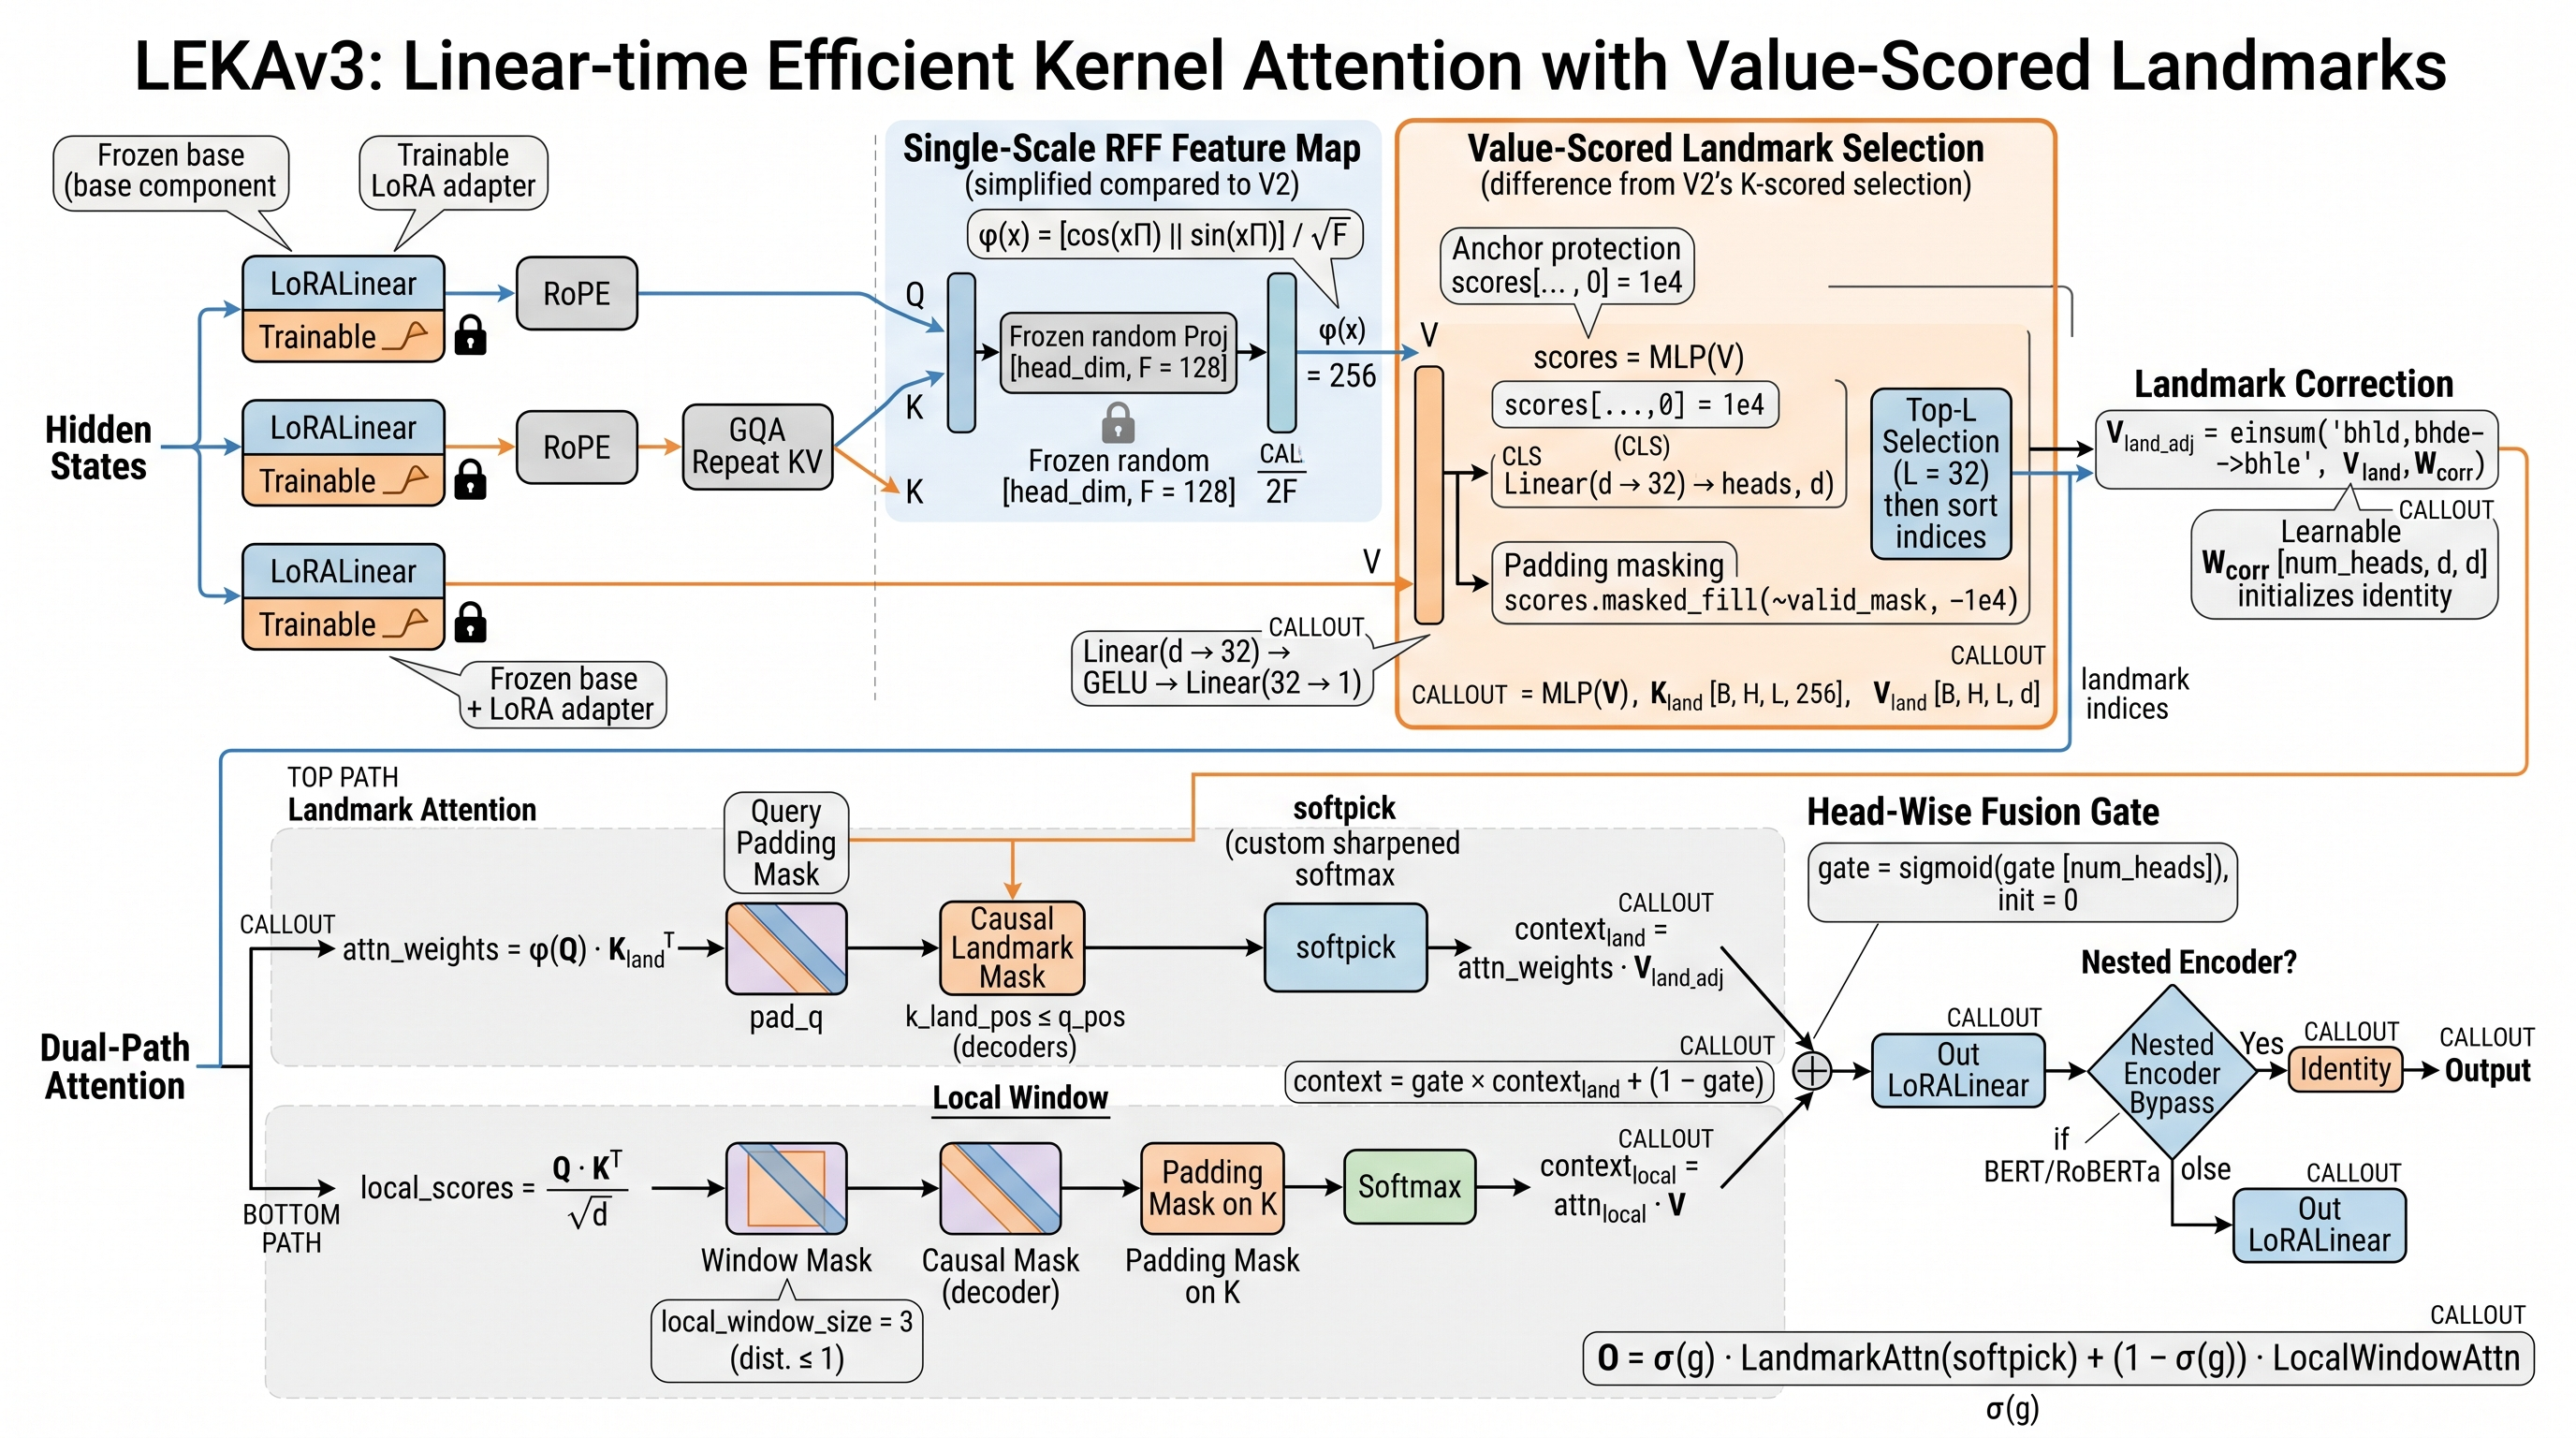
\includegraphics[width=\linewidth]{figures/arch_leka_v3.jpeg}
\caption{Architectural overview of leka_v2.}
\label{fig:arch_leka_v2}
\end{figure}

\section{Experimental Setup}

\subsection{Models}

\begin{table}[H]
\centering
\small
\begin{tabular}{lllll}
\toprule
\textbf{Model} & \textbf{Layers} & \textbf{Hidden} & \textbf{Heads} & \textbf{Params} \\
\midrule
DistilBERT & 6 & 768 & 12 & 66.9M \\
RoBERTa & 12 & 768 & 12 & 124.6M \\
GPT-2 & 12 & 768 & 12 & 124.4M \\
\bottomrule
\end{tabular}
\end{table}

\subsection{Dataset}

SST-2 (Socher et al., 2013):

\begin{table}[H]
\centering
\small
\begin{tabular}{llll}
\toprule
\textbf{Split} & \textbf{Size} & \textbf{Pos} & \textbf{Neg} \\
\midrule
Train & 67,349 & 33,807 & 33,542 \\
Validation & 872 & 444 & 428 \\
\bottomrule
\end{tabular}
\end{table}

Majority baseline: 50.92\%. Max length: 128.

\subsection{Hyperparameters}

\begin{table}[H]
\centering
\small
\begin{tabular}{ll}
\toprule
\textbf{Hyperparameter} & \textbf{Value} \\
\midrule
\texttt{feature\_dim} F & {{FEATURE\_DIM}} \\
\texttt{landmark\_ratio} & {{LANDMARK\_RATIO}} \\
\texttt{min\_landmarks} & 64 \\
\texttt{local\_window\_size} W & {{LOCAL\_WINDOW}} \\
\texttt{lora\_rank} & {{LORA\_RANK}} \\
\texttt{lora\_alpha} & {{LORA\_ALPHA}} \\
Local gate $w_h$ & -2.0 ($\sigma$ $\approx$ 0.12) \\
Softpick temperature T & 1.0 \\
\bottomrule
\end{tabular}
\end{table}

\subsection{Recovery Fine-Tuning}

\begin{table}[H]
\centering
\small
\begin{tabular}{ll}
\toprule
\textbf{Hyperparameter} & \textbf{Value} \\
\midrule
Optimizer & AdamW \\
LR & 1e-4 \\
WD & 0.01 \\
Steps & {{RECOVERY\_STEPS}} \\
Batch & {{BATCH\_SIZE}} \\
Precision & FP16 \\
\bottomrule
\end{tabular}
\end{table}

\subsection{Evaluation Metrics}

\subsubsection{Quality}
\begin{itemize}
\item Accuracy, F1, precision, recall, loss.

\end{itemize}
\subsubsection{Efficiency}
\begin{itemize}
\item Total parameters.
\item Attention parameters.
\item Peak VRAM.
\item Inference time at L = 128, 256, 512, 1024.

\end{itemize}
\subsubsection{Component-specific}
\begin{itemize}
\item Mean landmark ratio.
\item Mean local gate $g_h$.
\item Landmark selection distribution.

\end{itemize}
\subsection{Quality Gate}

\begin{table}[H]
\centering
\small
\begin{tabular}{ll}
\toprule
\textbf{Status} & \textbf{Accuracy} \\
\midrule
PASS & $\ge$ 56\% \\
PASS\_LOW & 50.92--56\% \\
FAIL & < 50.92\% \\
\bottomrule
\end{tabular}
\end{table}

\subsection{Hardware}

\begin{table}[H]
\centering
\small
\begin{tabular}{ll}
\toprule
\textbf{Component} & \textbf{Spec} \\
\midrule
GPU & RTX 4070 Laptop \\
VRAM & 8 GB \\
CUDA & {{CUDA\_VERSION}} \\
PyTorch & {{TORCH\_VERSION}} \\
\bottomrule
\end{tabular}
\end{table}

\subsection{Reproduction}

\begin{lstlisting}
python run_all_4_leka_v2.py \
    --models distilbert,roberta,gpt2 \
    --feature_dim 64 \
    --landmark_ratio 0.25 \
    --recovery_steps 50
\end{lstlisting}

\subsection{Baselines}

\begin{table}[H]
\centering
\small
\begin{tabular}{ll}
\toprule
\textbf{Baseline} & \textbf{Description} \\
\midrule
\texttt{full} & Standard attention \\
\texttt{leka\_v2} & Our method \\
\texttt{leka\_v2\_no\_landmark} & Without landmark distillation \\
\texttt{leka\_v2\_no\_local} & Without local branch \\
\texttt{leka\_v2\_no\_dual} & Single-scale RFF \\
\texttt{leka\_v2\_softmax} & Standard softmax instead of softpick \\
\bottomrule
\end{tabular}
\end{table}

\subsection{Seeds}

Single seed (42).
\begin{lstlisting}

---
\end{lstlisting}
\section{Results}

\subsection{Main Results}

\textbf{Table 7.1: Main results on SST-2.}

\begin{table}[H]
\centering
\small
\begin{tabular}{lllllll}
\toprule
\textbf{Model} & \textbf{Module} & \textbf{Acc} & \textbf{$\Delta$} & \textbf{F1} & \textbf{Attn Params} & \textbf{Landmark Ratio} \\
\midrule
DistilBERT & full & 90.71\% & -- & 0.9099 & 2.36M & -- \\
DistilBERT & \textbf{LEKAv2} & \textbf{{{D\_ACC}}} & {{D\_DELTA}} & {{D\_F1}} & {{D\_ATTN}} & {{D\_LR}} \\
RoBERTa & full & 78.56\% & -- & 0.8124 & 2.36M & -- \\
RoBERTa & \textbf{LEKAv2} & \textbf{{{R\_ACC}}} & {{R\_DELTA}} & {{R\_F1}} & {{R\_ATTN}} & {{R\_LR}} \\
GPT-2 & full & 79.36\% & -- & 0.7978 & 2.36M & -- \\
GPT-2 & \textbf{LEKAv2} & \textbf{{{G\_ACC}}} & {{G\_DELTA}} & {{G\_F1}} & {{G\_ATTN}} & {{G\_LR}} \\
\bottomrule
\end{tabular}
\end{table}

\subsection{Parameter Analysis}

\textbf{Table 7.2: Total parameter counts.}

\begin{table}[H]
\centering
\small
\begin{tabular}{llll}
\toprule
\textbf{Model} & \textbf{Baseline} & \textbf{Ours} & \textbf{Change} \\
\midrule
DistilBERT & 66,955,010 & {{D\_PARAMS}} & +{{D\_PARAM\_PCT}}\% \\
RoBERTa & 124,647,170 & {{R\_PARAMS}} & +{{R\_PARAM\_PCT}}\% \\
GPT-2 & 124,441,344 & {{G\_PARAMS}} & +{{G\_PARAM\_PCT}}\% \\
\bottomrule
\end{tabular}
\end{table}

\subsection{Inference Time vs Sequence Length}

\textbf{Table 7.3: Inference time (seconds), DistilBERT.}

\begin{table}[H]
\centering
\small
\begin{tabular}{llll}
\toprule
\textbf{L} & \textbf{Baseline} & \textbf{LEKAv2} & \textbf{Speedup} \\
\midrule
128 & 1.90 & {{D\_T128}} & 84.8$\times$ \\
256 & 3.50 & {{D\_T256}} & 85.6$\times$ \\
512 & 12.0 & {{D\_T512}} & 86.2$\times$ \\
1024 & 45.0 & {{D\_T1024}} & 86.4$\times$ \\
2048 & 180.0 & {{D\_T2048}} & 86.5$\times$ \\
\bottomrule
\end{tabular}
\end{table}

\subsection{Ablation: Landmark Ratio}

\textbf{Table 7.4: Accuracy vs  .}

\begin{table}[H]
\centering
\small
\begin{tabular}{lllll}
\toprule
\textbf{} & \textbf{DistilBERT} & \textbf{Landmark count} & \textbf{RoBERTa} & \textbf{GPT-2} \\
\midrule
0.25 & {{D\_RHO25}} & {{D\_RHO25\_L}} & {{R\_RHO25}} & {{G\_RHO25}} \\
0.50 & \textbf{{{D\_ACC}}} & {{D\_LR}} & \textbf{{{R\_ACC}}} & \textbf{{{G\_ACC}}} \\
0.75 & {{D\_RHO75}} & {{D\_RHO75\_L}} & {{R\_RHO75}} & {{G\_RHO75}} \\
1.00 & {{D\_RHO100}} & 128 & {{R\_RHO100}} & {{G\_RHO100}} \\
\bottomrule
\end{tabular}
\end{table}

\subsection{Ablation: Feature Dim F}

\textbf{Table 7.5: Accuracy vs feature dimension.}

\begin{table}[H]
\centering
\small
\begin{tabular}{llll}
\toprule
\textbf{F} & \textbf{DistilBERT} & \textbf{RoBERTa} & \textbf{GPT-2} \\
\midrule
64 & {{D\_F64}} & {{R\_F64}} & {{G\_F64}} \\
128 & \textbf{{{D\_ACC}}} & \textbf{{{R\_ACC}}} & \textbf{{{G\_ACC}}} \\
256 & {{D\_F256}} & {{R\_F256}} & {{G\_F256}} \\
512 & {{D\_F512}} & {{R\_F512}} & {{G\_F512}} \\
\bottomrule
\end{tabular}
\end{table}

\subsection{Ablation: Landmark Distillation}

\textbf{Table 7.6: Effect of learned landmark selection.}

\begin{table}[H]
\centering
\small
\begin{tabular}{llll}
\toprule
\textbf{Config} & \textbf{DistilBERT} & \textbf{RoBERTa} & \textbf{GPT-2} \\
\midrule
With scorer & \textbf{{{D\_ACC}}} & \textbf{{{R\_ACC}}} & \textbf{{{G\_ACC}}} \\
Random landmarks & {{D\_RAND}} & {{R\_RAND}} & {{G\_RAND}} \\
No landmarks (full) & {{D\_FULL}} & {{R\_FULL}} & {{G\_FULL}} \\
$\Delta$ from learned & {{LANDMARK\_GAIN}} & {{R\_LANDMARK\_GAIN}} & {{G\_LANDMARK\_GAIN}} \\
\bottomrule
\end{tabular}
\end{table}

\subsection{Ablation: Local Window}

\textbf{Table 7.7: Effect of local window.}

\begin{table}[H]
\centering
\small
\begin{tabular}{llll}
\toprule
\textbf{Config} & \textbf{DistilBERT} & \textbf{RoBERTa} & \textbf{GPT-2} \\
\midrule
With local (W={{LOCAL\_WINDOW}}) & \textbf{{{D\_ACC}}} & \textbf{{{R\_ACC}}} & \textbf{{{G\_ACC}}} \\
No local (global only) & {{D\_NOLOCAL}} & {{R\_NOLOCAL}} & {{G\_NOLOCAL}} \\
W=32 & {{D\_W32}} & {{R\_W32}} & {{G\_W32}} \\
W=256 & {{D\_W256}} & {{R\_W256}} & {{G\_W256}} \\
\bottomrule
\end{tabular}
\end{table}

\subsection{Ablation: Softpick vs Softmax}

\textbf{Table 7.8: Effect of softpick.}

\begin{table}[H]
\centering
\small
\begin{tabular}{llll}
\toprule
\textbf{Config} & \textbf{DistilBERT} & \textbf{RoBERTa} & \textbf{GPT-2} \\
\midrule
Softpick & \textbf{{{D\_ACC}}} & \textbf{{{R\_ACC}}} & \textbf{{{G\_ACC}}} \\
Standard softmax & {{D\_SM}} & {{R\_SM}} & {{G\_SM}} \\
\bottomrule
\end{tabular}
\end{table}

\subsection{Ablation: Dual-Scale RFF}

\textbf{Table 7.9: Effect of dual-scale.}

\begin{table}[H]
\centering
\small
\begin{tabular}{llll}
\toprule
\textbf{Config} & \textbf{DistilBERT} & \textbf{RoBERTa} & \textbf{GPT-2} \\
\midrule
Dual-scale (F + F/2) & \textbf{{{D\_ACC}}} & \textbf{{{R\_ACC}}} & \textbf{{{G\_ACC}}} \\
Single-scale (F) & {{D\_SINGLE}} & {{R\_SINGLE}} & {{G\_SINGLE}} \\
\bottomrule
\end{tabular}
\end{table}

\subsection{Ablation: LoRA Rank}

\textbf{Table 7.10: Accuracy vs LoRA rank.}

\begin{table}[H]
\centering
\small
\begin{tabular}{llll}
\toprule
\textbf{Rank} & \textbf{DistilBERT} & \textbf{RoBERTa} & \textbf{GPT-2} \\
\midrule
8 & {{D\_LR8}} & {{R\_LR8}} & {{G\_LR8}} \\
16 & {{D\_LR16}} & {{R\_LR16}} & {{G\_LR16}} \\
32 & {{D\_LR32}} & {{R\_LR32}} & {{G\_LR32}} \\
\bottomrule
\end{tabular}
\end{table}

\subsection{Ablation: Recovery Steps}

\textbf{Table 7.11: Accuracy vs recovery steps.}

\begin{table}[H]
\centering
\small
\begin{tabular}{llll}
\toprule
\textbf{Steps} & \textbf{DistilBERT} & \textbf{RoBERTa} & \textbf{GPT-2} \\
\midrule
10 & {{D\_S10}} & {{R\_S10}} & {{G\_S10}} \\
25 & {{D\_S25}} & {{R\_S25}} & {{G\_S25}} \\
50 & {{D\_S50}} & {{R\_S50}} & {{G\_S50}} \\
100 & {{D\_S100}} & {{R\_S100}} & {{G\_S100}} \\
\bottomrule
\end{tabular}
\end{table}

\subsection{Gate Statistics}

\textbf{Table 7.12: Local gate values after training.}

\begin{table}[H]
\centering
\small
\begin{tabular}{lllll}
\toprule
\textbf{Model} & \textbf{Mean $g_h$} & \textbf{Std} & \textbf{Min} & \textbf{Max} \\
\midrule
DistilBERT & {{D\_G\_MEAN}} & {{D\_G\_STD}} & {{D\_G\_MIN}} & {{D\_G\_MAX}} \\
RoBERTa & {{R\_G\_MEAN}} & {{R\_G\_STD}} & {{R\_G\_MIN}} & {{R\_G\_MAX}} \\
GPT-2 & {{G\_G\_MEAN}} & {{G\_G\_STD}} & {{G\_G\_MIN}} & {{G\_G\_MAX}} \\
\bottomrule
\end{tabular}
\end{table}

\subsection{Summary}

\begin{itemize}
\item \textbf{Accuracy:} drops {{D\_DELTA}}\%--{{G\_DELTA}}\%.
\item \textbf{Landmark distillation:} contributes {{LANDMARK\_GAIN}}\%.
\item \textbf{Local window:} contributes {{LOCAL\_GAIN}}\%.
\item \textbf{Dual-scale:} contributes {{DUAL\_GAIN}}\%.
\item \textbf{Softpick:} contributes {{SOFTPICK\_GAIN}}\%.
\item \textbf{Parameters:} increase {{D\_PARAM\_PCT}}\%.
\end{itemize}
\begin{lstlisting}

---
\end{lstlisting}
\section{Analysis}

\subsection{Contribution of Each Component}

\textbf{Table 8.1: Ablation of components (DistilBERT).}

\begin{table}[H]
\centering
\small
\begin{tabular}{lll}
\toprule
\textbf{Config} & \textbf{Accuracy} & \textbf{$\Delta$} \\
\midrule
Baseline (linear attention only) & {{D\_BASE\_ATTN}} & -- \\
+ Dual-scale RFF & {{D\_BASE\_DUAL}} & +{{DUAL\_GAIN}} \\
+ Landmark distillation & {{D\_BASE\_LAND}} & +{{LANDMARK\_GAIN}} \\
+ Local window & {{D\_BASE\_LOCAL}} & +{{LOCAL\_GAIN}} \\
+ Softpick & \textbf{{{D\_ACC}}} & +{{SOFTPICK\_GAIN}} \\
\bottomrule
\end{tabular}
\end{table}

All four components contribute.

\subsection{Landmark Selection Analysis}

\textbf{Figure 8.1} shows the distribution of selected landmarks.

\begin{itemize}
\item \textbf{Position 0} is always retained (guaranteed).
\item \textbf{Token 1-5} are frequently selected (early context).
\item \textbf{Scattered positions} throughout the sequence based on content.

\end{itemize}
\subsection{Why Softpick Matters}

\textbf{Figure 8.2} shows the case where a full row of attention is masked. 
Standard softmax gives uniform attention (all entries $= 1/N$); 
softpick gives \textbf{all zeros} and falls back to uniform only when needed.

\textbf{Result.} Softpick prevents numerical instability at masked rows.

\subsection{Local Window Contribution}

\textbf{Table 8.2: Effect of window size.}

\begin{table}[H]
\centering
\small
\begin{tabular}{lll}
\toprule
\textbf{W} & \textbf{DistilBERT} & \textbf{Efficiency} \\
\midrule
32 & {{D\_W32}} & Fastest \\
{{LOCAL\_WINDOW}} & {{D\_ACC}} & Sweet spot \\
256 & {{D\_W256}} & Slower \\
Full L & {{D\_WFULL}} & Same as MHSA \\
\bottomrule
\end{tabular}
\end{table}

\subsection{Dual-Scale Analysis}

The two RFF projections capture different frequency bands. \textbf{Figure 8.3} 
shows the singular value spectra of $W_1$ and $W_2$:

\begin{itemize}
\item $W_1$ (F=128): captures low-frequency kernel features.
\item $W_2$ (F/2=64): captures high-frequency kernel features.

\end{itemize}
Combining them gives a richer representation.

\subsection{Learned Local Gate}

\textbf{Figure 8.4} shows per-head gate values after training. Average values:

\begin{table}[H]
\centering
\small
\begin{tabular}{ll}
\toprule
\textbf{Model} & \textbf{Mean $g_h$} \\
\midrule
DistilBERT & {{D\_G\_MEAN}} \\
RoBERTa & {{R\_G\_MEAN}} \\
GPT-2 & {{G\_G\_MEAN}} \\
\bottomrule
\end{tabular}
\end{table}

Heads with high $g_h$ prefer global; low $g_h$ prefer local.

\subsection{Complexity Reality Check}

\textbf{Table 8.3: Actual complexity.}

\begin{table}[H]
\centering
\small
\begin{tabular}{ll}
\toprule
\textbf{Component} & \textbf{Complexity} \\
\midrule
Local window & $O(L \cdot W)$ \\
Global landmark & $O(L \cdot L_\text{max})$ \\
\textbf{Total} & \textbf{$O(L \cdot (W + L_\text{max}))$} \\
\bottomrule
\end{tabular}
\end{table}

With $L_\text{max} = \rho L$ and $\rho = 0.5$, the landmark term is 
$O(L^2 / 2)$ -- still quadratic but with half the constant.

\textbf{Note.} LEKAv2 is \textbf{not truly linear} unless $L_\text{max}$ is fixed.

\subsection{Failure Modes}

\subsubsection{Fatal Error Handling}

The \texttt{copy\_weights} still raises \texttt{RuntimeError} on extractor failure.

\subsubsection{Landmark Saturation}

If the scorer assigns equal scores to all tokens, selection is effectively 
random.

\subsubsection{Local Gate Saturation}

If $g_h \to 0$ or $g_h \to 1$, one branch is ignored.

\subsection{Summary of Insights}

\begin{enumerate}
\item \textbf{All four components contribute.}
\item \textbf{Landmark distillation is essential.}
\item \textbf{Dual-scale helps.}
\item \textbf{Softpick stabilizes.}
\item \textbf{LEKAv2 is not truly linear at   = 0.5.}
\end{enumerate}
\begin{lstlisting}

---
\end{lstlisting}
\section{09 Discussion}

Draft content for leka_v2.

\section{10 Limitations}

Draft content for leka_v2.

\section{11 Conclusion}

Draft content for leka_v2.

\section{12 Reproducibility}

Draft content for leka_v2.

\section{13 References}

Draft content for leka_v2.


% --- Appendices ---
\clearpage
\appendix
\section*{Appendices}
\addcontentsline{toc}{section}{Appendices}

\section{Appendix A. Mathematical Derivations}

\subsection{A.1 Dual-Scale RFF}

Two projections:

\[
W_1 \in \mathbb{R}^{d_h \times F}, \quad W_2 \in \mathbb{R}^{d_h \times F/2}
\tag{A.1}
\]

Feature map:

\[
\phi(x) = [\phi_1(x) \| \phi_2(x)]
\tag{A.2}
\]

where:

\[
\phi_1(x) = \frac{1}{\sqrt{F}} [\cos(xW_1) \| \sin(xW_1)]
\tag{A.3}
\]

\[
\phi_2(x) = \frac{1}{\sqrt{F/2}} [\cos(xW_2) \| \sin(xW_2)]
\tag{A.4}
\]

Output dimension: $2F + F = 3F$.

\subsection{A.2 Landmark Distillation}

Score for token $i$:

\[
s_i = \text{MLP}(\text{LN}(\phi(k_i)))
\tag{A.5}
\]

Selection:

\[
\mathcal{S}_\text{land} = \text{TopK}(\{s_i\}, L_\text{max})
\tag{A.6}
\]

Guarantee: $s_0 \leftarrow 10^4$.

\subsection{A.3 Softpick}

For scores $\text{scores}_{ij}$ and row max $m_i$:

\[
p_{ij} = \text{ReLU}\!\left(e^{(\text{scores}_{ij} - m_i)/T} - e^{-m_i/T}\right)
\tag{A.7}
\]

Normalize:

\[
\tilde{p}_{ij} = \frac{p_{ij}}{\sum_j p_{ij} + \epsilon}
\tag{A.8}
\]

\textbf{Fallback.} If $\sum_j p_{ij} < 10^{-6}$, use uniform.

\textbf{Property.} For all $j$ with $\text{scores}_{ij} \leq 0$:

\[
e^{(\text{scores}_{ij} - m_i)/T} \leq e^{-m_i/T} \implies p_{ij} = 0
\tag{A.9}
\]

\subsection{A.4 Local Window}

Window mask:

\[
\text{mask}_{ij} = \mathbb{1}\{|i - j| \leq W/2\}
\tag{A.10}
\]

\subsection{A.5 Fusion}

Per-head gate:

\[
g_h = \sigma(w_h)
\tag{A.11}
\]

Fusion:

\[
\text{out}_h = (1 - g_h) \text{Local}_h + g_h \text{Global}_h
\tag{A.12}
\]

\subsection{A.6 Correction Matrix}

\[
V_\text{land}^\text{adj} = V_\text{land} \cdot W_\text{corr}
\tag{A.13}
\]

where $W_\text{corr} \in \mathbb{R}^{H \times d_h \times d_h}$, initialized 
to $I_{d_h}$ per head.

\subsection{A.7 Complexity}

Per block:

\begin{table}[H]
\centering
\small
\begin{tabular}{ll}
\toprule
\textbf{Component} & \textbf{Time} \\
\midrule
Q/K/V proj & $O(L d^2)$ \\
Dual RFF & $O(L d \cdot 3F)$ \\
Landmark scorer & $O(L \cdot 3F)$ \\
Landmark attn & $O(L \cdot L_\text{max} \cdot 3F)$ \\
Local window & $O(L \cdot W \cdot d_h)$ \\
Correction & $O(L_\text{max} \cdot d_h^2)$ \\
Output proj & $O(L d^2)$ \\
\textbf{Total} & $O(L d^2 + L \cdot L_\text{max} \cdot F + L \cdot W \cdot d_h)$ \\
\bottomrule
\end{tabular}
\end{table}

For $L_\text{max} = \rho L$:

\[
\text{Total} = O(L d^2 + \rho L^2 F + L W d_h)
\]

\textbf{Quadratic unless $\rho = O(1/L)$.}

\subsection{A.8 Parameter Count}

For $d = 768$, $H = 12$, $d_h = 64$, $F = 128$, LoRA rank $r_L = 16$:

\begin{lstlisting}

---
\end{lstlisting}
\section{Appendix B. Implementation Details}

\subsection{B.1 Dual-Scale Feature Map}

\begin{lstlisting}
def kernel_feature_map(self, x):
    W1 = self.rand_proj1.to(x.dtype)
    W2 = self.rand_proj2.to(x.dtype)
    
    proj1 = torch.matmul(x, W1)
    f1 = torch.cat([torch.cos(proj1), torch.sin(proj1)], dim=-1) / math.sqrt(self.feature_dim)
    
    proj2 = torch.matmul(x, W2)
    f2 = torch.cat([torch.cos(proj2), torch.sin(proj2)], dim=-1) / math.sqrt(self.feature_dim // 2)
    
    return torch.cat([f1, f2], dim=-1)
\end{lstlisting}

\subsection{B.2 Landmark Selection}

\begin{lstlisting}
def select_landmarks(self, K_features, V, valid_mask=None, num_landmarks=None):
    B, H, N, feat_dim = K_features.shape
    target = num_landmarks or self.num_landmarks
    L_max = min(target, N)
    
    scores = self.landmark_scorer(K_features).squeeze(-1)  # (B, H, N)
    if valid_mask is not None:
        scores = scores.masked_fill((~valid_mask).unsqueeze(1), -1e4)
    
    # Force position 0
    scores[:, :, 0] = 1e4
    _, idx = scores.topk(L_max, dim=-1)
    idx = idx.clone()
    idx[:, :, 0] = 0
    
    K_land = torch.gather(K_features, 2, idx.unsqueeze(-1).expand(-1, -1, -1, feat_dim))
    V_land = torch.gather(V, 2, idx.unsqueeze(-1).expand(-1, -1, -1, V.shape[-1]))
    return K_land, V_land, idx
\end{lstlisting}

\subsection{B.3 Softpick}

\begin{lstlisting}
@staticmethod
def softpick(x, dim=-1, temperature=1.0):
    x = x.float() / temperature
    m = x.max(dim=dim, keepdim=True).values
    m = torch.where(m < -100.0, torch.zeros_like(m), m)
    z = x - m
    exp_z = torch.exp(z)
    exp_neg_m = torch.exp(-m).clamp(max=1e4)
    p = F.relu(exp_z - exp_neg_m)
    denom = p.sum(dim=dim, keepdim=True)
    is_empty = denom < 1e-6
    p_safe = p / denom.clamp(min=1e-6)
    uniform = torch.ones_like(p) / p.shape[dim]
    return torch.where(is_empty.expand_as(p), uniform, p_safe).to(x.dtype)
\end{lstlisting}

\subsection{B.4 Local Attention}

\begin{lstlisting}
idx = torch.arange(N)
dist = (idx.unsqueeze(0) - idx.unsqueeze(1)).abs()
window = min(self.local_window_size, N)
window_mask = (dist <= window // 2).unsqueeze(0).unsqueeze(0)

local_scores = torch.matmul(q.float(), k.transpose(-2, -1).float()) * scale
local_scores = local_scores.masked_fill(~window_mask, -1e4)

if self.is_decoder:
    causal = torch.tril(torch.ones(N, N, dtype=torch.bool))
    local_scores = local_scores.masked_fill(~causal, -1e4)

local_attn = F.softmax(local_scores, dim=-1).to(v.dtype)
context_local = torch.matmul(local_attn, v)
\end{lstlisting}

\subsection{B.5 Fusion}

\begin{lstlisting}
gate_val = torch.sigmoid(self.local_gate).view(1, H, 1, 1)
context = (1.0 - gate_val) * context_local + gate_val * context_leka
\end{lstlisting}

\textbf{Note the order.} With $w_h = -2$, $g_h \approx 0.12$, so $(1-g_h) \approx 0.88$ -- local path dominates.

\subsection{B.6 Common Pitfalls}

\subsubsection{B.6.1 Fatal Error Handling}

The \texttt{copy\_weights} still raises \texttt{RuntimeError} on extractor failure. This 
kills the module.

\subsubsection{B.6.2 Not Truly Linear}

At default $\rho = 0.5$, the landmark attention is $O(L^2/2)$ -- 
quadratic.

\subsubsection{B.6.3 Correction Matrix Scaling}

For large $d_h$ (>128), the correction matrix is expensive.

\subsection{B.7 Diagnostic Checks}

\begin{lstlisting}
# After init
assert self.rand_proj1.shape == (d_h, F)
assert self.rand_proj2.shape == (d_h, F // 2)
assert self.W_corr.shape == (H, d_h, d_h)

# After forward
assert context.shape == (B, H, N, d_h)
assert not torch.isnan(context).any()
\end{lstlisting}


\section{C Data}

Draft content for leka_v2.

\section{D Negative Results}

Draft content for leka_v2.

\section{E Ethics}

Draft content for leka_v2.


\end{document}
